\addchapheadtotoc
\chapter{Results and Discussion}
In this chapter we describe the experiments conducted in this work and discuss the results. Most of these experiments were performed on a synthetic graph dataset based on the stochastic block model (SBM). Considering a generative model allows to control the difficulty of the graph classification problem. The SBM is widely used to model real world datasets \citep{SBM}.

We first compare the various random features scheme proposed in this work, particularly in terms of computational time. Then, we examine how the algorithm $GSA-\varphi_{OPU}$ with optical random features, followed by a support vector machine model (SVM), is affected by the various parameters: the sampling technique, the number of samples $s$, the graphlet size $k$ and the number of random features $m$.
We then benchmark this algorithm against state-of-the-art methods: graphlet kernel and graph convolutional networks (GCN). %In addition, we benchmark it to $GSA-\varphi_{Gs}$.
Finally, we show some experiments on a real world dataset (DD). 
We point out here that the OPU we used is developed by a company, LightOn, located in Paris. We collaborated with this company for this work, where for all the experiments, an OPU was accessed remotely for computation.

Let us start by a general introduction to the generative SBM model.
 
\section{Stochastic block model (SBM) dataset}

SBM is commonly known in social sciences to model group structures in friendship graph networks \citep{SBM}. The basic idea is that nodes are clustered into different communities. Then, edges between nodes are randomly drawn such that nodes in the same community have a higher probability of being connected than nodes in different communities.

Formally, to generate a graph $\G=(\V,\E)$ of size $v$, the following parameters should be given: the number of communities $\eta$ in the graph, the community labels of the nodes $\{b_1 , \ldots ,b_v\}$ such that node $u$ belongs to community $b_u$, and a symmetric edge probability matrix $\mathbf{P}=(p_{i,j})_{i,j\in\{1,\ldots, \eta\}} \in [0,1]^{\eta \times \eta}$.
Then the graph is generated by independently adding an edge between any two pair of nodes $(u_1,u_2)$ with probability $p_{b_{u_1} , b_{u_2}}$.

\begin{figure}[H]
\centering
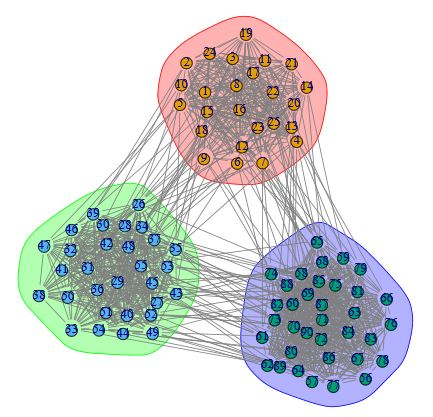
\includegraphics[scale=0.5]{SBM.JPG}
\caption[Visualization of an SBM-based graph example]{An example of a graph generated using SBM model, the graph has 90 nodes divided into three communities of size 25, 30 and 35 nodes. An edge between two nodes within the same community has a probability 0.8, while it has a probability 0.5 if the two nodes belong to different communities.}
%Source:
\label{fig:SBM_example}
\end{figure}

Note that the average degree $\mu_u$ of any node $u$ is given by:
\begin{equation}
    \mu_u=\Big[\sum_{b_i\neq b_u} p_{b_u,b_i}*(\#\{ u'\in \V, b_{u'}=b_i \} )\Big]+p_{b_u,b_u}*(\#\{u'\in \V, b_{u'}=b_u \}-1 )
\end{equation}

\subsection{Dataset setup}

In every experiment, unless otherwise mentioned, we generate a SBM dataset consisting of 300 graphs, 240 as a training set and 60 as a test set. Each graph has $v=60$ nodes divided equally between six communities $\eta=6$. Moreover, graphs are divided into two classes based on two different choices of the matrix $\mathbf{P}$. For the class $j\in\{0,1\}$, the matrix $\mathbf{P}_j$ contains $p_{in,j}$ on its diagonal as the intra-community edge probability and $p_{out,j}$ outside its diagonal.


In order to prevent the two classes from being easily discriminated by the average degree of nodes in the graph as a feature, the two pairs of probabilities $(p_{in,j}, p_{out,j})$ are chosen such that all nodes have a fixed expected average degree equal to $\mu=10$. We denote by $r=(p_{in,1}/p_{in,0})$ the inter-classes similarity parameter: the closer $r$ is to $1$, the more similar both classes are, and thus the harder it is to discriminate them. We fix $p_{in,0} = 0.3$, and therefore the only parameter adjusted in the experiments is $r$.

\subsection{Histogram visualization}
Let us quickly visualize what are the histograms $\mathbf{f}_\G$ of graphlets that are manipulated by the classical graphlet kernel for our SBM data. We generate a graph $\G$ by SBM with a randomly chosen pair $(p_{in},p_{out})$, then we compare the following: exhaustive enumeration of all size-5 graphlets in $\G$, sampling $s=2000$ graphlets of the same size with uniform sampling, or sampling 2000 graphlets using random walks. For each case, we built using $\varphi^{match}_k$ a histogram of graphlets \emph{without repetition}. We show the three graphlet histograms in Fig. \ref{fig:graphlet_hist}. 

\begin{figure}[H]
\centering
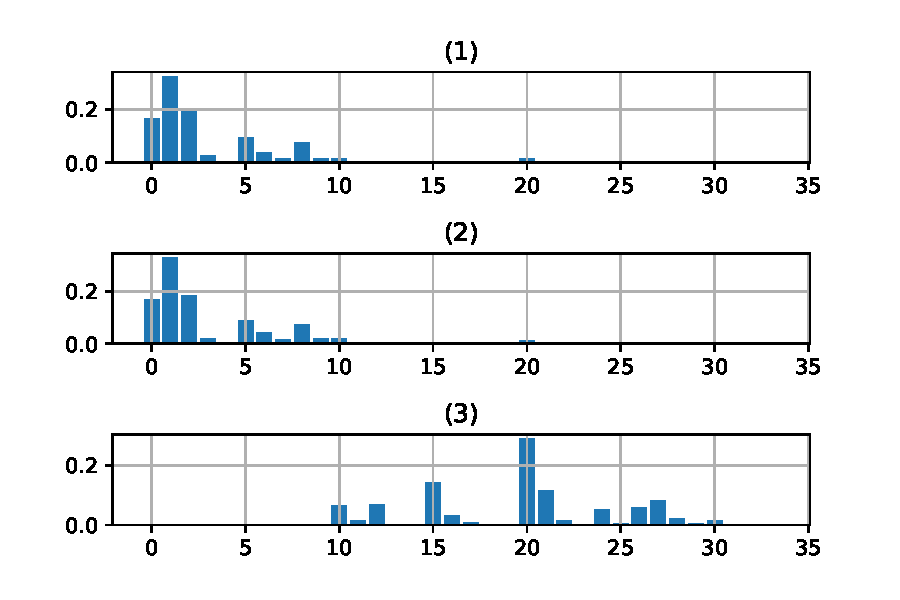
\includegraphics[scale=0.7]{class0_hist.pdf}
\caption[Graphlet histograms of uniform and random walk sampling techniques]{Size-5 graphlet histograms (wihtout repetition) of an SBM random graph. (1): With exhaustive enumeration of all graphlets. (2): 2000 samples with uniform sampling. (3): 2000 samples using random walk sampling. }
%Source:
\label{fig:graphlet_hist}
\end{figure}

As expected, empirical uniform sampling provides a good approximation of exhaustive enumeration, and changing the sampling technique modifies the histogram. Moreover, we ordered the graphlets such that the more disconnected graphlets are on the left and the connected graphlets on the right, and as expected random walk sampling tends to produce more connected graphlets than uniform sampling. To be fair with the classical graphlet kernel, in all the following experiments we consider uniform sampling technique, unless otherwise mentioned.
\section{Choice of feature map $\varphi$ }
\label{section:choice}
In this section, we examine how the choice of $\varphi$ affects the performance and computation time of GSA-$\varphi$. Then we benchmark GSA-$\varphi_{OPU}$ against graphlet kernel. Finally, we plot the empirical computational time of each algorithm. 

\textbf{Comparison of random features}: in this experiment we compare different random feature maps $\varphi$ in our algorithm. For this experiment we have the following parameters:  inter-class similarity $r=1.1$, graphlet size $k=6$, and samples number $s=2000$. The bandwidth parameter of the Gaussian kernel is empirically selected as $\sigma=0.1$.

\begin{figure}[h]
\centering
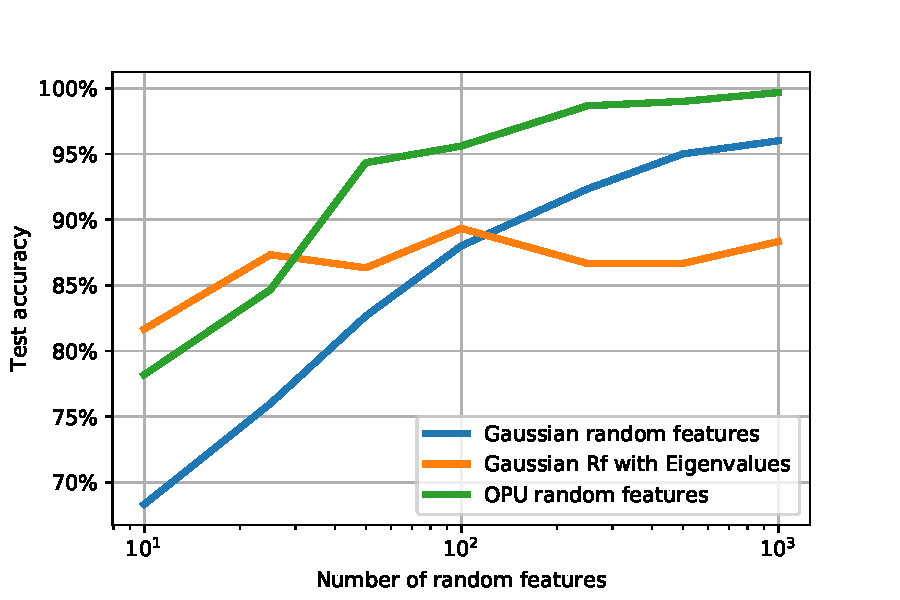
\includegraphics[scale=0.6]{figs/phi_comparison.pdf}
\caption[Comparison between different $\varphi$ maps in $GSA-\varphi$]{Comparison between different $\varphi$ maps in $GSA-\varphi$: optical random features $\varphi_{OPU}$, gaussian random Fourier features $\varphi_{Gs}$, Gaussian random Fourier features on sorted eigenvalues $\varphi_{Gs+Eigen}$. Fixed parameters: $r=1.1$, $k=6$,  $s=2000$, and $\sigma=0.1$. We plot the test accuracy related to each $\varphi$ as a function of $m$.}
%Source:
\label{fig:phi_comparison}
\end{figure}
Preserving the same settings of the parameters and the dataset, we applied the optical random features $GSA-\varphi_{OPU}$ or Gaussian random features $GSA-\varphi_{Gs}$ directly on adjacency matrices, which do not respect graphlet isomorphism, and Gaussian random features on sorted eigenvalues $GSA-\varphi_{Gs+Eigen}$, which respect graphlet isomorphism. Then we plot the the test accuracies as a  function of the number of random features $m$ in Fig. \ref{fig:phi_comparison}.

We observe that $GSA-\varphi_{OPU}$ gives the best results on this experiment. On the contrary, $GSA-\varphi_{Gs+Eigen}$ performs best with a low number of random features, but increasing this number does not really improve the result and it is over-matched at high $m$. A possible justification is that the Eigenvalues of the adjacency matrix loses information about the graphlets, even though respecting the isomorphism means that we are working with a smaller histogram and less random features are required.

\textbf{\boldsymbol{$GSA-\varphi_{OPU}$} Vs. graphlet kernel} :
Here we compare between the performance of $GSA-\varphi_{OPU}$ and the graphlet kernel with graph sampling, that is, $GSA-\varphi$ with $\varphi = \varphi^{match}_k$ without repetition. We take the following parameters: number of random features $m=5000$, graphlet size $k$=5, and number of samples $s=2000$ (for both algorithms). We run both experiments while we vary the value of inter-class similarity parameter $r$, and we plot the test accuracy in Fig. \ref{fig:gk_vs_opu}.

\begin{figure}[H]
\centering
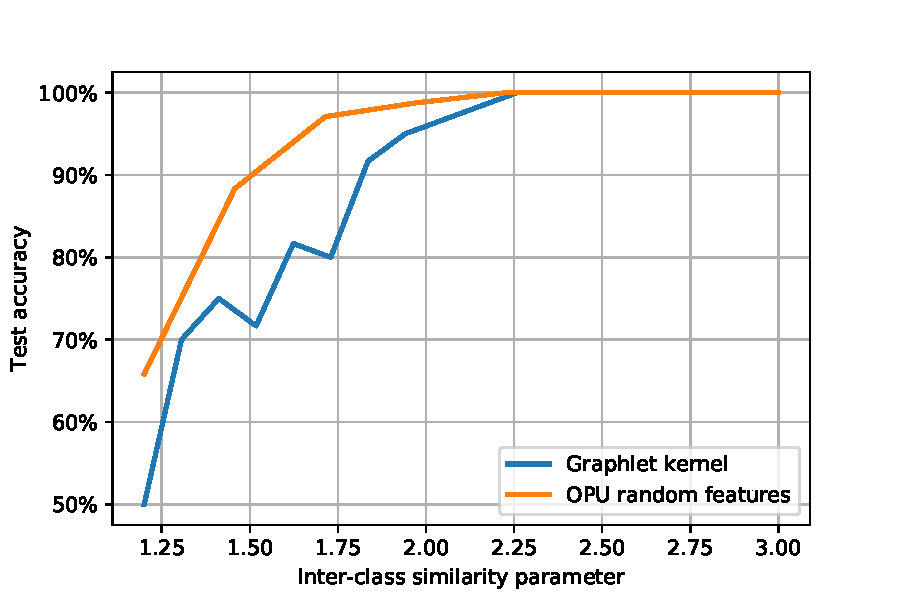
\includegraphics[scale=0.6]{figs/gk_vs_opu.pdf}
\caption[graphlet kernel Vs $GSA-\varphi_{OPU}$  ]{graphlet kernel Vs $GSA-\varphi_{OPU}$   }
%Source:
\label{fig:gk_vs_opu}
\end{figure}
We see that with the same limited number of samples, $GSA-\varphi_{OPU}$ clearly outperforms the graphlet kernel with matching function. We conclude that the mean kernel induced by the OPU is more adapted in this case than the traditional graphlet kernel. %thus it outperforms the traditional graphlet kernel if both algorithms consider exhaustive enumeration of graphlets.

\textbf{Computational time}
The same aforementioned experiments in this section are repeated with different graphlet size $k$. This is done to check how the computational time required by each grows in $k$. Results are shown in Fig. \ref{fig:computational_comparison}.
\begin{figure}[H]
\centering
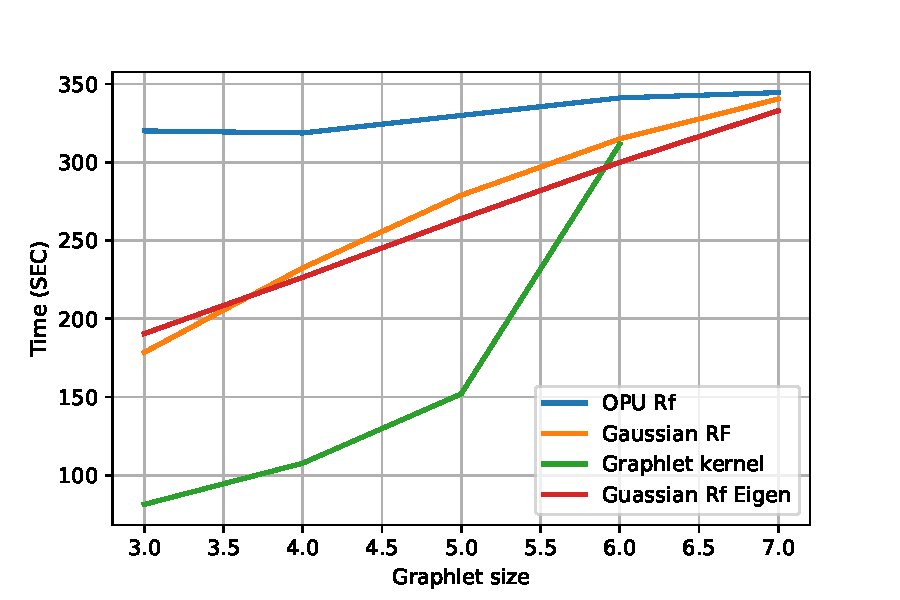
\includegraphics[scale=0.6]{figs/computational_comp.pdf}
\caption[Comparison in Computational cost between methods  ]{Comparison between different methods with respect to Computational cost  }
%Source:
\label{fig:computational_comparison}
\end{figure}

As expected, the execution time of the graphlet kernel with matching function grows exponentially with the graphlet size $k$, and polynomial for $GSA-\varphi_{Gs}$ and $GSA-\varphi_{Gs+Eigen}$. On the contrary, it is almost constant for $GSA-\varphi_{OPU}$, where the slight variation are due to overhead computation and not the feature map itself. We should point out here that, with the current settings, there is a significant overhead between the point in time where we run our optimizer code on the OPUs server and the point when the OPU actually launches the computation. To be fair, this overhead computation time should be precisely measured and substracted from $GSA-\varphi_{OPU}$ execution time. As the technology comes into maturity, we can expect this additional time to be significantly reduced. 

To summarize, $GSA-\varphi_{OPU}$ outperforms the traditional graphlet sampling both in accuracy and computational cost.

\section{Role of each parameter in $GSA-\varphi_{OPU}$}

In this section, we perform various experiments to examine the role of each parameter of GSA-$\varphi$ on the classification performance, using the optical random features $\varphi_{OPU}$.

\subsection{Number of samples $s$}
We first examine the minimum number of samples needed to classify both classes with high test accuracy.% (also called validation accuracy).
%
%\subsection{Varying the number of samples $s$}
 We use the following parameters: number of random features $m=5000$, and inter-class similarity $r=2$. These parameters were chosen such that the two classes can be efficiently classified with sufficiently large $s$ and large $k$. Then for three graphlet sizes $k\in\{4,5,6\}$, we vary the number of samples and plot the test accuracy in Fig. \ref{fig:varying_samples_num}.

 %To understand this we can consider the critical case when we use $k=1$ between two graphs, which means that we count how many nodes there are in each. Obviously this is a redundant choice since such graphlets don't provide a lot of information on how nodes are structured and connected in the graph. Thus, for each application, we must choose large $k$ so that graphlets include discriminative patterns not useless ones.
\begin{figure}[H]
\centering
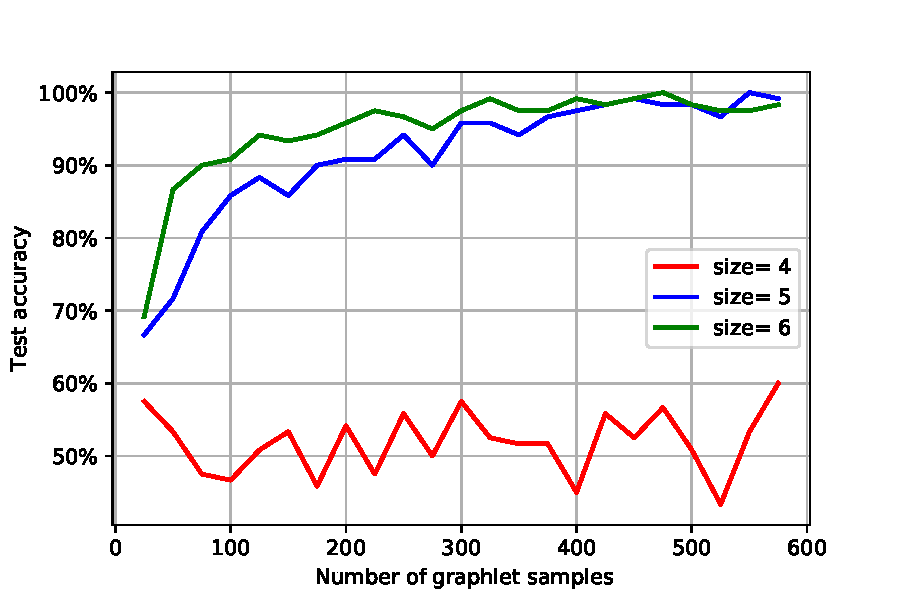
\includegraphics[scale=0.6]{figs/samples_num.pdf}
\caption[$GSA-\varphi_{OPU}$ behavior with respect to number of samples $s$]{$GSA-\varphi_{OPU}$ behavior with respect to number of samples $s$. With $r=2$, $m=5000$, $k\in\{4,5,6\}$, and uniform sampling.}
%Source:
\label{fig:varying_samples_num}
\end{figure}
Results show that, in these settings, even with large number of samples the algorithm will not perform well if the graphlet size is too small. It is known that the algorithm is strictly more powerful for high graphlet size (for instance, $k=2$ only computes the density of edges), and it seems that here $k=4$ is unsufficient. %Secondly, %is that in this experiment and even in the next ones, we don't have access to apply the kernel which corresponds to OPUS' random features. That's why we cannot get sure that these results meets the concentration inequalities in chapter\ref{chapter:fast_algorithm}. 
However, we see that for $k\in\{5,6\}$, test accuracy increases as $s$ increases, and that a fairly low number of samples is enough to obtain good classification results. As shown in the previous sections, with higher number of samples the performance of the algorithm converges to the performance of the corresponding algorithm with exhaustive sampling.

\subsection{Number of random features $m$}
In this experiment we explore the role of random features number $m$ in our algorithm. 
We take the following parameters: inter-class similarity $r=1.1$, graphlet size $k=6$, samples number $s=2000$, and uniform sampling.
In addition, for every value of $m$, we repeated the experiment $5$ times, and plot both individual results and average accuracies in Fig. \ref{fig:varying_random_features}. We can see that when $m$ grows, the average test accuracy gets higher. Moreover, as $m$ increases, the 5 experiments provide lower-variance accuracies, which is compatible with the concentration inequalities in chapter \ref{chapter:fast_algorithm}, as at high $m$ we approximate the performance of the mean kernel.

\begin{figure}[H]
\centering
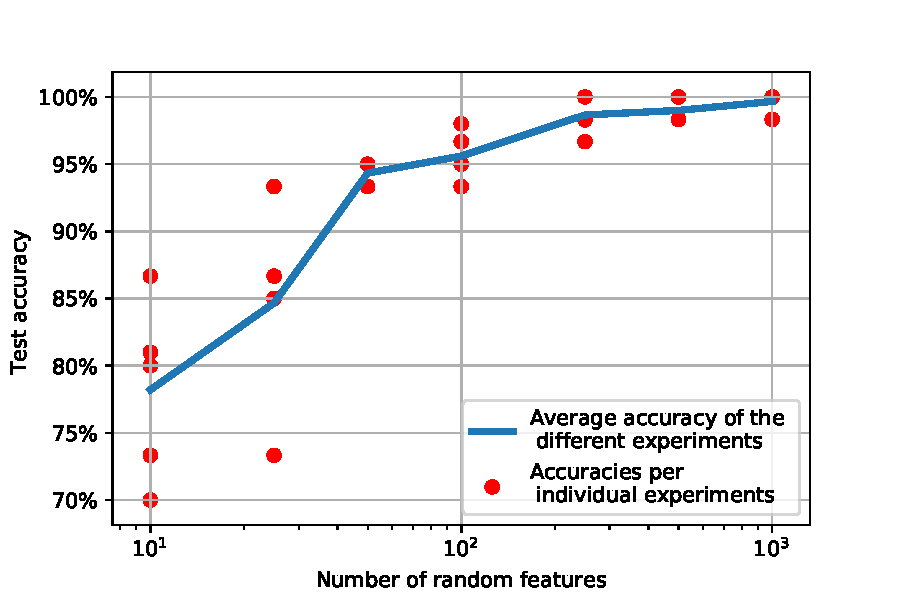
\includegraphics[scale=0.6]{figs/LightON_adj_SBM_varying_RF.PDF}
\caption[$GSA-\varphi_{OPU}$ behavior with respect to number of random features $m$]{$GSA-\varphi_{OPU}$ behavior with respect to number of random features $m$. With $r=1.1$, $k=6$, $s=2000$. For every value of $m$, the experiment is repeated five times (red dots), then the $5$ resulted accuracies are averaged (blue curve).}
\label{fig:varying_random_features}
\end{figure}

\subsection{Sampling method}
Now we explore the role of the sampling technique in our algorithm. We take a sample number $s=2000$.
Then for three graphlet sizes $k\in\{3,4,5,6\}$, we vary the value of inter-classes similarity parameter $r$ and plot the test accuracy of both uniform and random walk sampling techniques, as shown in Fig. \ref{fig:comp_sampling}.
\begin{figure}
     \centering
     \begin{subfigure}[b]{0.49\textwidth}
         \centering
         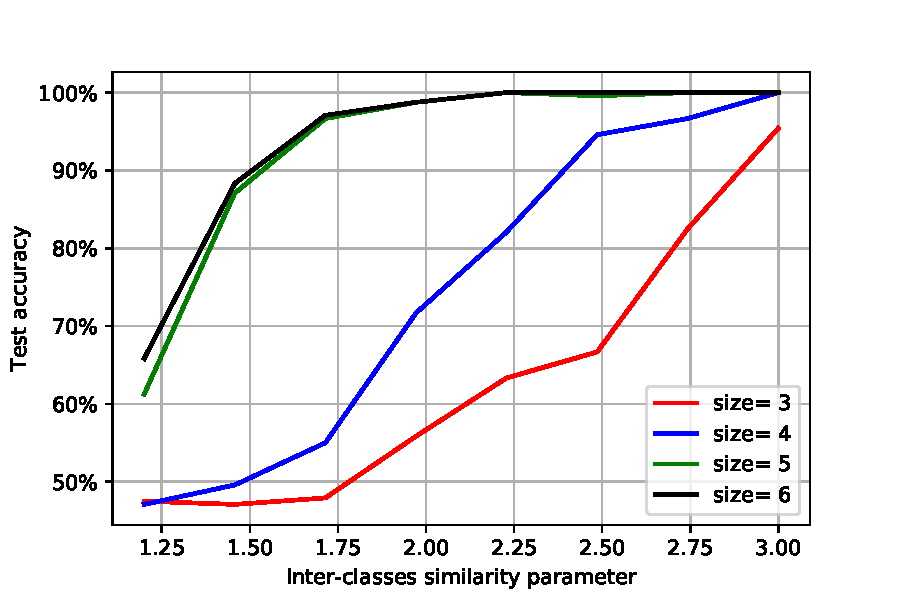
\includegraphics[width=\textwidth]{figs/LightOn_adj_SBM_Similarity_graphlet_size.pdf}
         \caption{Uniform sampling}
         \label{fig:y equals x}
     \end{subfigure}
     \hfill
     \begin{subfigure}[b]{0.49\textwidth}
         \centering
         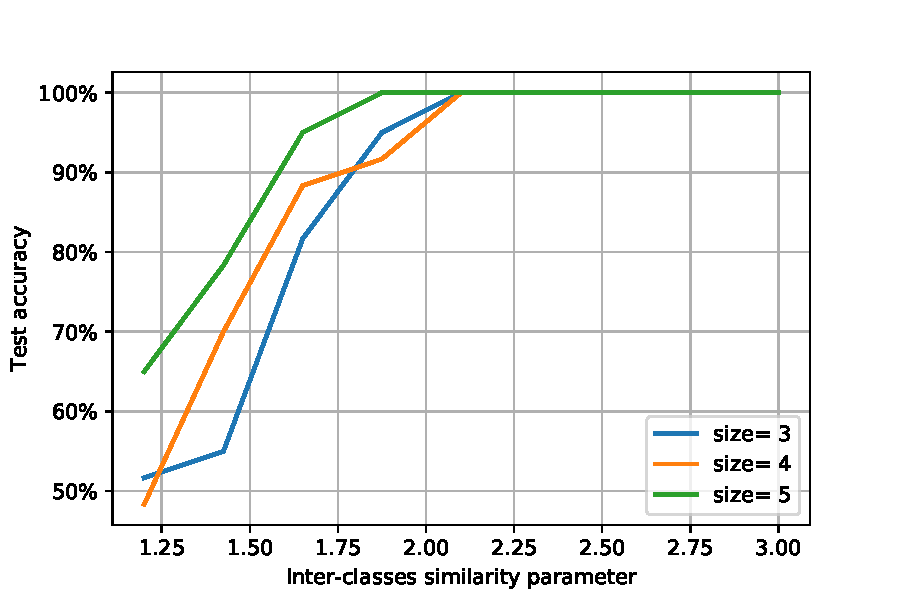
\includegraphics[width=\textwidth]{figs/LightOn_adj_SBM_similarity_graphlet_size_RW.pdf}
         \caption{Random walk sampling}
         \label{fig:three sin x}
     \end{subfigure}
        \caption [$GSA-\varphi_{OPU}$ behavior with respect to sampling technique]{$GSA-\varphi_{OPU}$ behavior with respect to sampling technique. With $m=5000$, $s=2000$, we vary the value of $r$ and plot the test accuracy of the algorithm when using uniform and random walk samplers. This is done for different graphlet sizes.}
%Source:
\label{fig:comp_sampling}
\end{figure}
Results show that for graphlet sizes $>5$, both sampling techniques perform similarly well. For uniform sampling, however, we note a gap between curves that correspond to $k=4$ and $k=5$, which we do not observe for the random walk sampler. This might be justified by the tendency of uniform sampling to produce disconnected graphlets, which is accentuated at low graphlet size, since one has less chance of encountering an existing edge than for large graphlets. This is not the case for random walk. A careful analysis of this phenomenon will be done in future work.

\section{Comparison with graph convolution networks}
In this section, we compare $GSA-\varphi_{OPU}$ with a Graph Neural Network architecture. We modified and trained one model based on GIN (Graph Isomorphism Network) \citep{GCN_powerful}, which has been reported to give excellent results on many graph classification tasks.
The chosen model consists of 5 GIN layers followed by two fully connected layers where the dimensions of hidden layers are equal to 4. 

In this experiment, we trained then tested this model on our dataset with trying different values of inter-classes similarity parameter $r$, and results are shown in Fig. \ref{fig:GCN_GIN_SBM_multfactor_RW}, where we also recall the results for $GSA-\varphi_{OPU}$ with random walk sampling.

\begin{figure}[h]
\centering
     \begin{subfigure}[b]{0.49\textwidth}
         \centering
         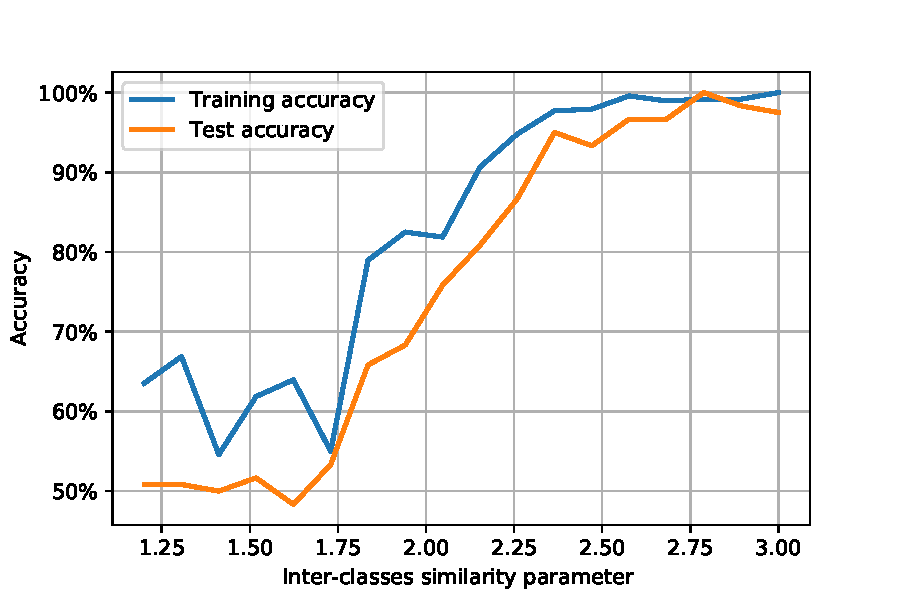
\includegraphics[width=\textwidth]{figs/GCN.pdf}
         \caption{Graph Isomorphism Network}
         \label{subfig:GIN}
     \end{subfigure}
     \hfill
     \begin{subfigure}[b]{0.49\textwidth}
         \centering
         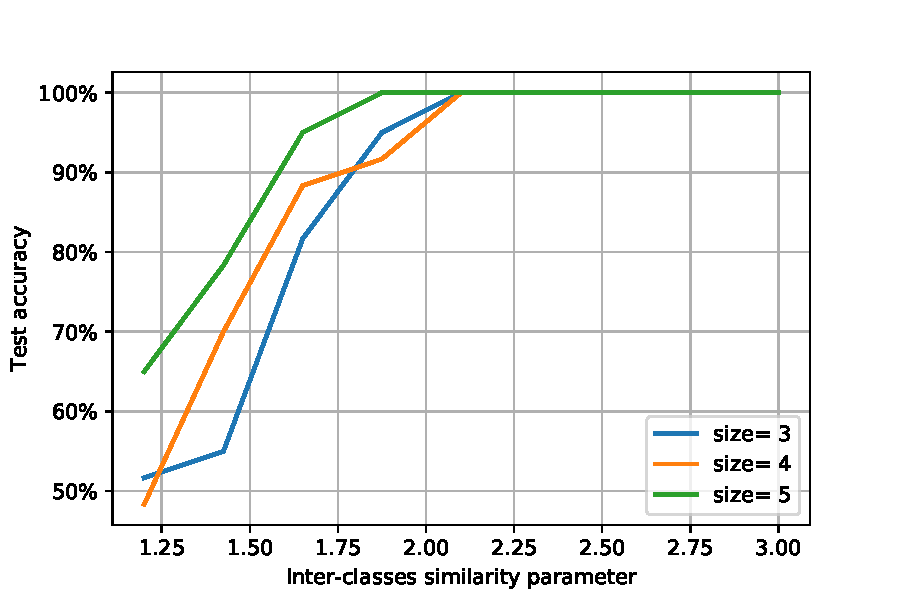
\includegraphics[width=\textwidth]{figs/LightOn_adj_SBM_similarity_graphlet_size_RW.pdf}
         \caption{$GSA-\varphi_{OPU}$ with random walk sampling}
         \label{subfig:GSAvsGIN}
     \end{subfigure}
\caption[GCN model's classification test accuracy as a function of Inter-classes similarity parameter ]{GCN model's classification test accuracy with respect to Inter-classes similarity parameter.}
%Source:
\label{fig:GCN_GIN_SBM_multfactor_RW}
\end{figure}
Comparing GCN to $GSA-\varphi_{OPU}$, we can see that performs better performs better when the graphlet size is greater than 4, especially using  random walk sampling technique. We note that we do not report the computational time for GIN, since it is highly dependent on high-speed graphical processing units (GPUs) to do the training process. %, thus we cannot compare both algorithms from computational-time point of view.

\section{Results on D\&D dataset}
D\&D is a dataset of size $n=1178$ graphs, each graph represents a protein structures \citep{DD_ref}. The nodes represent amino acids and two nodes are connected by an edge if they are less than 6 Angstroms apart. The problem  is to classify the protein structures into enzymes and non-enzymes. We note that in the original dataset each node has 7 features, which are not used by our algorithms, \emph{i.e.} we will try to classify the graphs just based on their structure. Using node features is without doubt necessary to reach state-of-the-art results, our goal here is mainly to test our algorithm on real data as a proof of concept.

We do the experiment with graphlet size $k=7$, samples number $s=4000$, and varying $m$.
For every value of $m$, we repeat the experiment $5$ times with different feature map and different training/testing division of the dataset, and plot both individual results and average accuracies in Fig. \ref{fig:DD}. %We can see that when $m$ grows, the average test accuracy gets higher, \emph{i.e.} we approximate the performance of the original mean kernel. Even further, as $m$ increases, the 5 experiments provide lower-variance accuracies, which is compatible with the concentration inequalities in chapter \ref{chapter:fast_algorithm}.
Although we do not observe a clear, steady average improvement in accuracy when $m$ grows, the results of the 5 corresponding experiments get more concentrated around the average value, giving a desirable reduced variance between experiments. On the other hand, at low $m$ accuracy results show high variance between experiments, which might be accentuated by the fact that nodes features are ignored. %However, it was interesting to touch the need to incorporate both sides of information.

\begin{figure}[H]
\centering
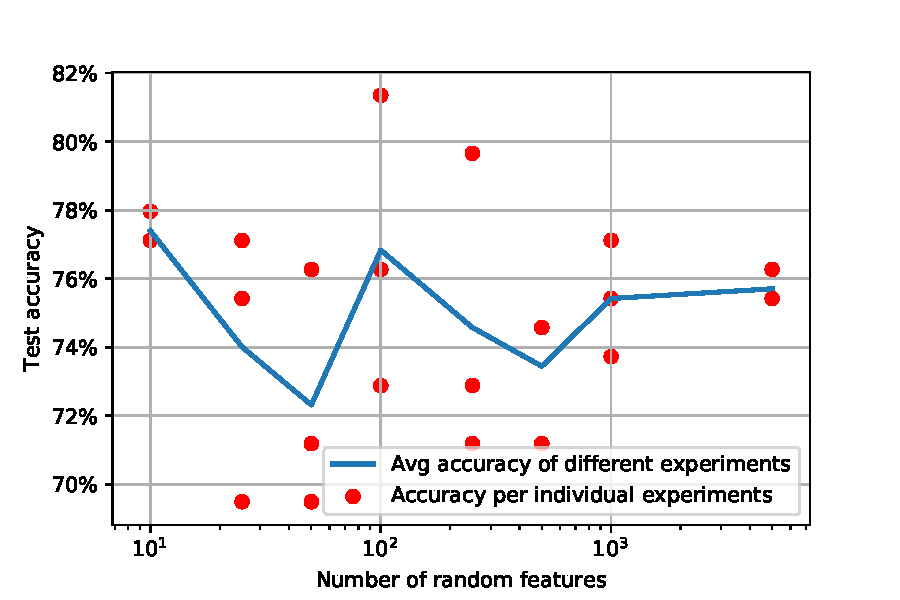
\includegraphics[scale=0.6]{figs/DD.pdf}
\caption[$GSA-\varphi_{OPU}$ results on D\&D dataset]{$GSA-\varphi_{OPU}$ results on D\&D. With  $k=7$, $s=4000$. For every value of $m$, the experiment is done five times (red dots), then the $5$ resulted accuracies are averaged (blue curve).}
\label{fig:DD}
\end{figure}


\section{Conclusion and future work}
Graph kernels were for a long of time part of the tools used in graph classification learning methods. However, many of them suffer from high computational time, especially the well known \emph{graphlet kernel}. In this work, we propose  new algorithms which, combined with efficient random projections, overcome this limitation. Inspired by graphlet kernel with graph sampling, we propose a family of algorithm that combines graph sampling with efficient mappings instead of graphlet matching, which requires an expensive isomorphism test. Then, we proposed to choose this mapping as kernel random features, and related the method with the mean kernel methodology and related MMD metric, showing a concentration of the random embedding around this metric. Finally, while classical random features still require expensive matrix-vector multiplication, we used optical random features projections, which can be computed in constant time by a recently developed optical hardware based on coherent light scattering through opaque medium. The resulting algorithm has strictly better computational complexity than the graphlet kernel, while concentrating around a well-defined MMD metric. Experiments on real and synthetic data show that it is significantly faster than traditional graphlet kernel and generally performs better. Furthermore, in our settings it even performed better than a particular graph convolutional networks on graph classification.

\textbf{Future work:} A major point left open to be analyzed is how to use our algorithm to classify graphs with node features. It is known that graph convolutional networks (GCN) have limits in learning just from the graph structure. So, one promising possibility is to use our algorithm to generate features embeddings on the graph level, and then feed these embeddings with the nodes' features of the graph to a deep neural network. By doing this, we take advantage of the speed of both our algorithm and GPUs. On the theoretical side, the properties of our new MMD metric could be further analyzed on particular models of graphs.



